\documentclass[tikz,border=10pt]{standalone}
\usepackage{mathabx}
\usetikzlibrary{backgrounds}
\usepackage{newunicodechar}
\newunicodechar{♮}{$\natural$}
\newunicodechar{♭}{$\flat$}
\newunicodechar{♯}{$\sharp$}
\newunicodechar{➚}{$\nearrow$}
\newunicodechar{➘}{$\searrow$}
\newunicodechar{ʼ}{'}
\newunicodechar{Ȧ}{\stackon[0.8pt]{A}{.}}
\newunicodechar{Ḃ}{\stackon[0.8pt]{B}{.}}
\newunicodechar{Ċ}{\stackon[0.8pt]{C}{.}}
\newunicodechar{Ḋ}{\stackon[0.8pt]{D}{.}}
\newunicodechar{Ė}{\stackon[0.8pt]{E}{.}}
\newunicodechar{Ḟ}{\stackon[0.8pt]{F}{.}}
\newunicodechar{Ġ}{\stackon[0.8pt]{G}{.}}


\def\centerarc[#1](#2)(#3:#4:#5);%
{
  \draw[#1]([shift=(#3:#5)]#2) arc (#3:#4:#5);
}


\begin{document}
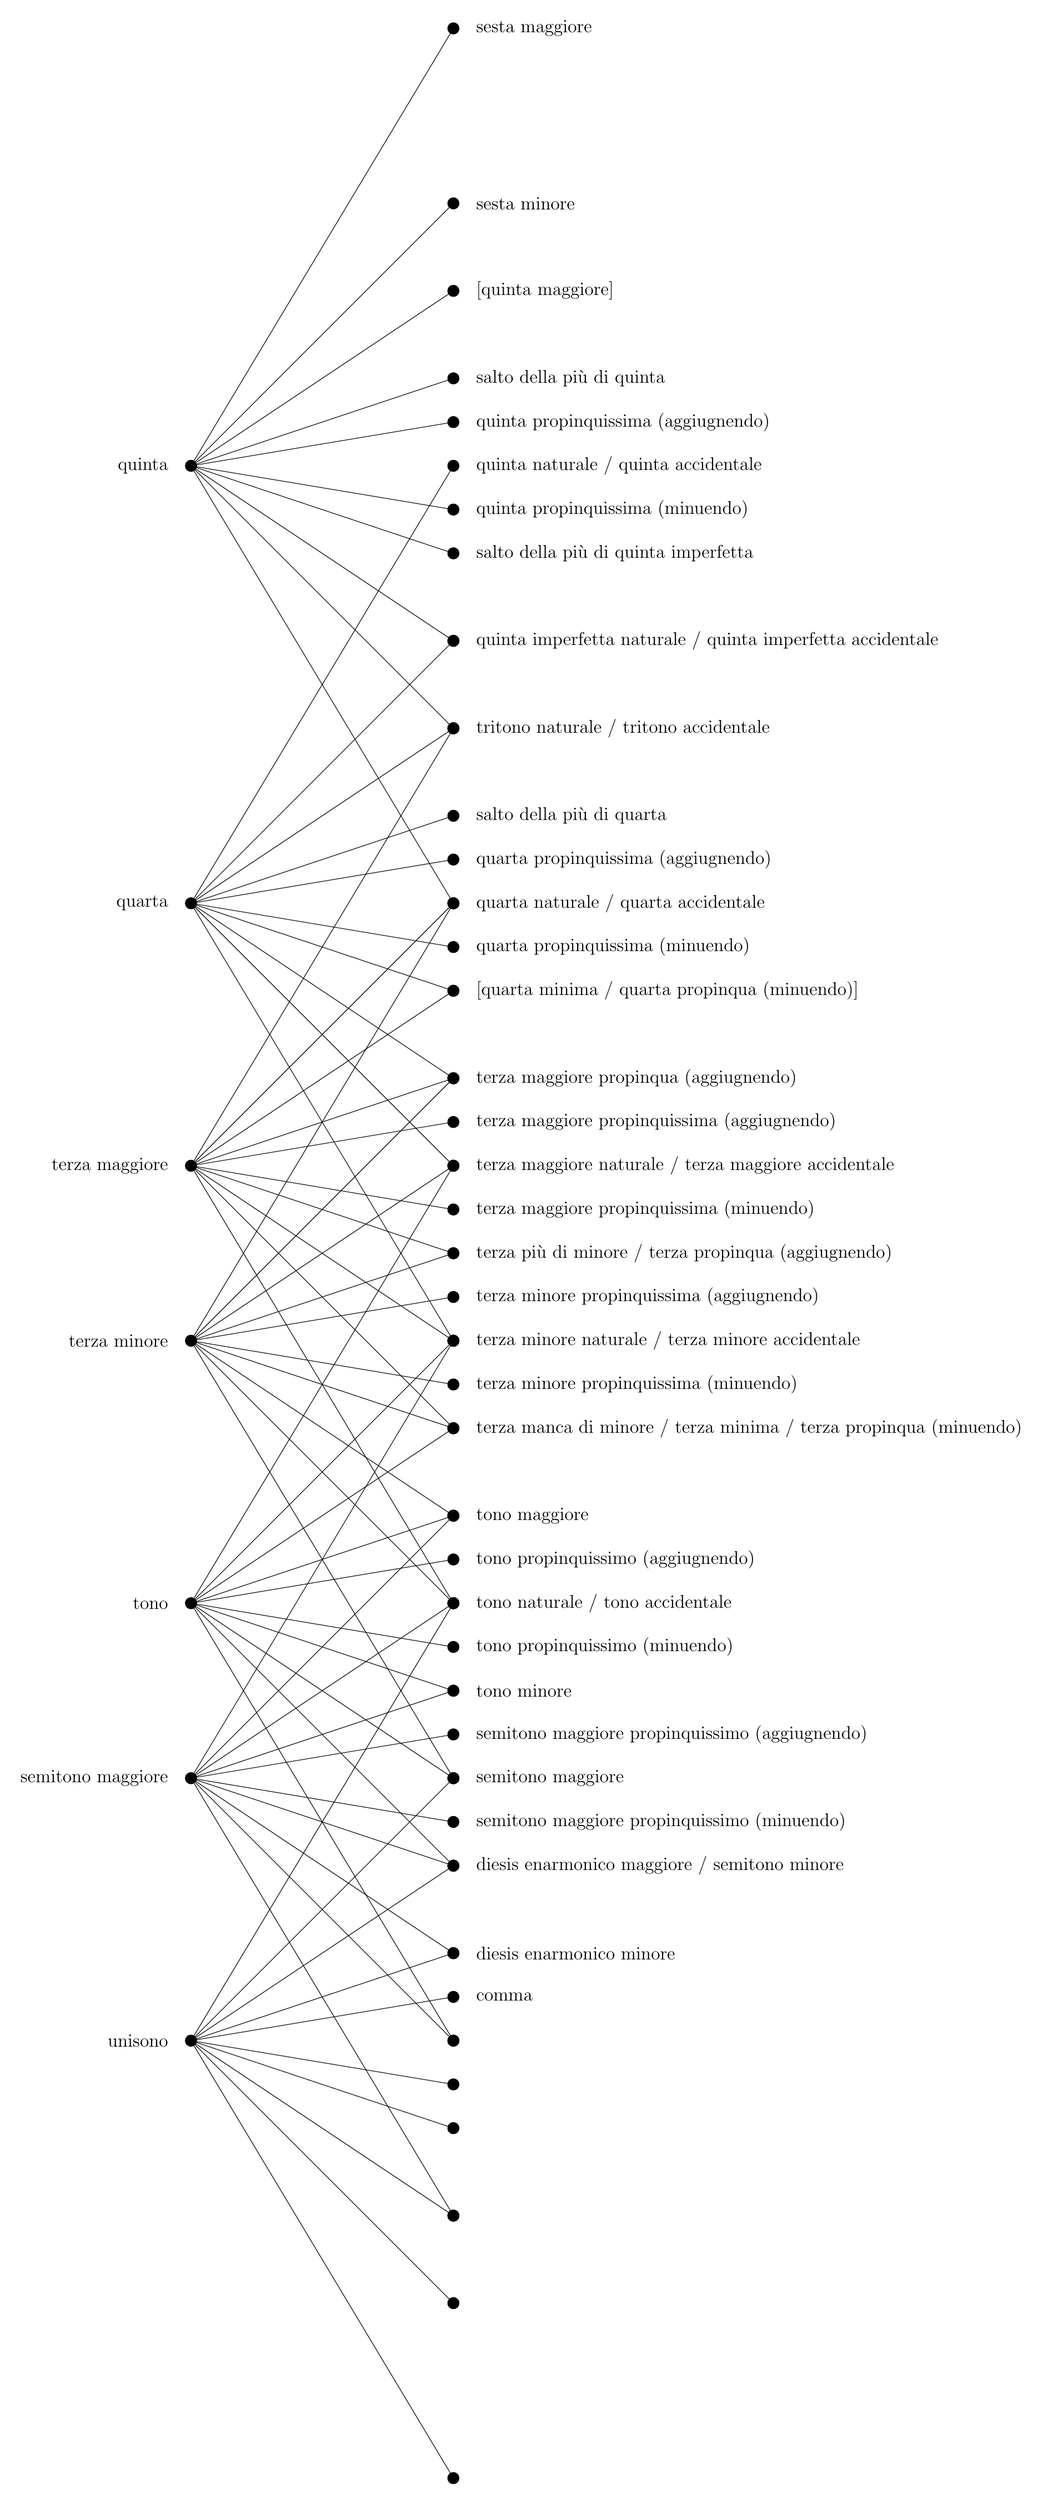
\begin{tikzpicture}

\draw (1.0,0.0) -- (7.0,1.0);
\draw (1.0,0.0) -- (7.0,-1.0);
\draw (1.0,0.0) -- (7.0,2.0);
\draw (1.0,0.0) -- (7.0,-2.0);
\draw (1.0,0.0) -- (7.0,4.0);
\draw (1.0,0.0) -- (7.0,-4.0);
\draw (1.0,0.0) -- (7.0,6.0);
\draw (1.0,0.0) -- (7.0,-6.0);
\draw (1.0,0.0) -- (7.0,10.0);
\draw (1.0,0.0) -- (7.0,-10.0);
\draw (1.0,6.0) -- (7.0,7.0);
\draw (1.0,6.0) -- (7.0,5.0);
\draw (1.0,6.0) -- (7.0,8.0);
\draw (1.0,6.0) -- (7.0,4.0);
\draw (1.0,6.0) -- (7.0,10.0);
\draw (1.0,6.0) -- (7.0,2.0);
\draw (1.0,6.0) -- (7.0,12.0);
\draw (1.0,6.0) -- (7.0,0.0);
\draw (1.0,6.0) -- (7.0,16.0);
\draw (1.0,6.0) -- (7.0,-4.0);
\draw (1.0,10.0) -- (7.0,11.0);
\draw (1.0,10.0) -- (7.0,9.0);
\draw (1.0,10.0) -- (7.0,12.0);
\draw (1.0,10.0) -- (7.0,8.0);
\draw (1.0,10.0) -- (7.0,14.0);
\draw (1.0,10.0) -- (7.0,6.0);
\draw (1.0,10.0) -- (7.0,16.0);
\draw (1.0,10.0) -- (7.0,4.0);
\draw (1.0,10.0) -- (7.0,20.0);
\draw (1.0,10.0) -- (7.0,0.0);
\draw (1.0,16.0) -- (7.0,17.0);
\draw (1.0,16.0) -- (7.0,15.0);
\draw (1.0,16.0) -- (7.0,18.0);
\draw (1.0,16.0) -- (7.0,14.0);
\draw (1.0,16.0) -- (7.0,20.0);
\draw (1.0,16.0) -- (7.0,12.0);
\draw (1.0,16.0) -- (7.0,22.0);
\draw (1.0,16.0) -- (7.0,10.0);
\draw (1.0,16.0) -- (7.0,26.0);
\draw (1.0,16.0) -- (7.0,6.0);
\draw (1.0,20.0) -- (7.0,21.0);
\draw (1.0,20.0) -- (7.0,19.0);
\draw (1.0,20.0) -- (7.0,22.0);
\draw (1.0,20.0) -- (7.0,18.0);
\draw (1.0,20.0) -- (7.0,24.0);
\draw (1.0,20.0) -- (7.0,16.0);
\draw (1.0,20.0) -- (7.0,26.0);
\draw (1.0,20.0) -- (7.0,14.0);
\draw (1.0,20.0) -- (7.0,30.0);
\draw (1.0,20.0) -- (7.0,10.0);
\draw (1.0,26.0) -- (7.0,27.0);
\draw (1.0,26.0) -- (7.0,25.0);
\draw (1.0,26.0) -- (7.0,28.0);
\draw (1.0,26.0) -- (7.0,24.0);
\draw (1.0,26.0) -- (7.0,30.0);
\draw (1.0,26.0) -- (7.0,22.0);
\draw (1.0,26.0) -- (7.0,32.0);
\draw (1.0,26.0) -- (7.0,20.0);
\draw (1.0,26.0) -- (7.0,36.0);
\draw (1.0,26.0) -- (7.0,16.0);
\draw (1.0,36.0) -- (7.0,37.0);
\draw (1.0,36.0) -- (7.0,35.0);
\draw (1.0,36.0) -- (7.0,38.0);
\draw (1.0,36.0) -- (7.0,34.0);
\draw (1.0,36.0) -- (7.0,40.0);
\draw (1.0,36.0) -- (7.0,32.0);
\draw (1.0,36.0) -- (7.0,42.0);
\draw (1.0,36.0) -- (7.0,30.0);
\draw (1.0,36.0) -- (7.0,46.0);
\draw (1.0,36.0) -- (7.0,26.0);
\draw[fill] (1.0,0.0) circle (0.13);
\draw[fill] (1.0,6.0) circle (0.13);
\draw[fill] (1.0,10.0) circle (0.13);
\draw[fill] (1.0,16.0) circle (0.13);
\draw[fill] (1.0,20.0) circle (0.13);
\draw[fill] (1.0,26.0) circle (0.13);
\draw[fill] (1.0,36.0) circle (0.13);
\node[anchor=east] at (0.6, 0.0) { \large unisono };
\node[anchor=east] at (0.6, 6.0) { \large semitono maggiore };
\node[anchor=east] at (0.6, 10.0) { \large tono };
\node[anchor=east] at (0.6, 16.0) { \large terza minore };
\node[anchor=east] at (0.6, 20.0) { \large terza maggiore };
\node[anchor=east] at (0.6, 26.0) { \large quarta };
\node[anchor=east] at (0.6, 36.0) { \large quinta };
\draw[fill] (7.0,26.0) circle (0.13);
\draw[fill] (7.0,46.0) circle (0.13);
\draw[fill] (7.0,30.0) circle (0.13);
\draw[fill] (7.0,42.0) circle (0.13);
\draw[fill] (7.0,32.0) circle (0.13);
\draw[fill] (7.0,40.0) circle (0.13);
\draw[fill] (7.0,34.0) circle (0.13);
\draw[fill] (7.0,38.0) circle (0.13);
\draw[fill] (7.0,35.0) circle (0.13);
\draw[fill] (7.0,37.0) circle (0.13);
\draw[fill] (7.0,16.0) circle (0.13);
\draw[fill] (7.0,36.0) circle (0.13);
\draw[fill] (7.0,20.0) circle (0.13);
\draw[fill] (7.0,32.0) circle (0.13);
\draw[fill] (7.0,22.0) circle (0.13);
\draw[fill] (7.0,30.0) circle (0.13);
\draw[fill] (7.0,24.0) circle (0.13);
\draw[fill] (7.0,28.0) circle (0.13);
\draw[fill] (7.0,25.0) circle (0.13);
\draw[fill] (7.0,27.0) circle (0.13);
\draw[fill] (7.0,10.0) circle (0.13);
\draw[fill] (7.0,30.0) circle (0.13);
\draw[fill] (7.0,14.0) circle (0.13);
\draw[fill] (7.0,26.0) circle (0.13);
\draw[fill] (7.0,16.0) circle (0.13);
\draw[fill] (7.0,24.0) circle (0.13);
\draw[fill] (7.0,18.0) circle (0.13);
\draw[fill] (7.0,22.0) circle (0.13);
\draw[fill] (7.0,19.0) circle (0.13);
\draw[fill] (7.0,21.0) circle (0.13);
\draw[fill] (7.0,6.0) circle (0.13);
\draw[fill] (7.0,26.0) circle (0.13);
\draw[fill] (7.0,10.0) circle (0.13);
\draw[fill] (7.0,22.0) circle (0.13);
\draw[fill] (7.0,12.0) circle (0.13);
\draw[fill] (7.0,20.0) circle (0.13);
\draw[fill] (7.0,14.0) circle (0.13);
\draw[fill] (7.0,18.0) circle (0.13);
\draw[fill] (7.0,15.0) circle (0.13);
\draw[fill] (7.0,17.0) circle (0.13);
\draw[fill] (7.0,0.0) circle (0.13);
\draw[fill] (7.0,20.0) circle (0.13);
\draw[fill] (7.0,4.0) circle (0.13);
\draw[fill] (7.0,16.0) circle (0.13);
\draw[fill] (7.0,6.0) circle (0.13);
\draw[fill] (7.0,14.0) circle (0.13);
\draw[fill] (7.0,8.0) circle (0.13);
\draw[fill] (7.0,12.0) circle (0.13);
\draw[fill] (7.0,9.0) circle (0.13);
\draw[fill] (7.0,11.0) circle (0.13);
\draw[fill] (7.0,-4.0) circle (0.13);
\draw[fill] (7.0,16.0) circle (0.13);
\draw[fill] (7.0,0.0) circle (0.13);
\draw[fill] (7.0,12.0) circle (0.13);
\draw[fill] (7.0,2.0) circle (0.13);
\draw[fill] (7.0,10.0) circle (0.13);
\draw[fill] (7.0,4.0) circle (0.13);
\draw[fill] (7.0,8.0) circle (0.13);
\draw[fill] (7.0,5.0) circle (0.13);
\draw[fill] (7.0,7.0) circle (0.13);
\draw[fill] (7.0,-10.0) circle (0.13);
\draw[fill] (7.0,10.0) circle (0.13);
\draw[fill] (7.0,-6.0) circle (0.13);
\draw[fill] (7.0,6.0) circle (0.13);
\draw[fill] (7.0,-4.0) circle (0.13);
\draw[fill] (7.0,4.0) circle (0.13);
\draw[fill] (7.0,-2.0) circle (0.13);
\draw[fill] (7.0,2.0) circle (0.13);
\draw[fill] (7.0,-1.0) circle (0.13);
\draw[fill] (7.0,1.0) circle (0.13);
\node[anchor=west] at (7.4, 1.0) { \large comma };
\node[anchor=west] at (7.4, 2.0) { \large diesis enarmonico minore };
\node[anchor=west] at (7.4, 4.0) { \large diesis enarmonico maggiore / semitono minore };
\node[anchor=west] at (7.4, 5.0) { \large semitono maggiore propinquissimo (minuendo) };
\node[anchor=west] at (7.4, 6.0) { \large semitono maggiore };
\node[anchor=west] at (7.4, 7.0) { \large semitono maggiore propinquissimo (aggiugnendo) };
\node[anchor=west] at (7.4, 8.0) { \large tono minore };
\node[anchor=west] at (7.4, 9.0) { \large tono propinquissimo (minuendo) };
\node[anchor=west] at (7.4, 10.0) { \large tono naturale / tono accidentale };
\node[anchor=west] at (7.4, 11.0) { \large tono propinquissimo (aggiugnendo) };
\node[anchor=west] at (7.4, 12.0) { \large tono maggiore };
\node[anchor=west] at (7.4, 14.0) { \large terza manca di minore / terza minima / terza propinqua (minuendo) };
\node[anchor=west] at (7.4, 15.0) { \large terza minore propinquissima (minuendo) };
\node[anchor=west] at (7.4, 16.0) { \large terza minore naturale / terza minore accidentale };
\node[anchor=west] at (7.4, 17.0) { \large terza minore propinquissima (aggiugnendo) };
\node[anchor=west] at (7.4, 18.0) { \large terza più di minore / terza propinqua (aggiugnendo) };
\node[anchor=west] at (7.4, 19.0) { \large terza maggiore propinquissima (minuendo) };
\node[anchor=west] at (7.4, 20.0) { \large terza maggiore naturale / terza maggiore accidentale };
\node[anchor=west] at (7.4, 21.0) { \large terza maggiore propinquissima (aggiugnendo) };
\node[anchor=west] at (7.4, 22.0) { \large terza maggiore propinqua (aggiugnendo) };
\node[anchor=west] at (7.4, 24.0) { \large [quarta minima / quarta propinqua (minuendo)] };
\node[anchor=west] at (7.4, 25.0) { \large quarta propinquissima (minuendo) };
\node[anchor=west] at (7.4, 26.0) { \large quarta naturale / quarta accidentale };
\node[anchor=west] at (7.4, 27.0) { \large quarta propinquissima (aggiugnendo) };
\node[anchor=west] at (7.4, 28.0) { \large salto della più di quarta };
\node[anchor=west] at (7.4, 30.0) { \large tritono naturale / tritono accidentale };
\node[anchor=west] at (7.4, 32.0) { \large quinta imperfetta naturale / quinta imperfetta accidentale };
\node[anchor=west] at (7.4, 34.0) { \large salto della più di quinta imperfetta };
\node[anchor=west] at (7.4, 35.0) { \large quinta propinquissima (minuendo) };
\node[anchor=west] at (7.4, 36.0) { \large quinta naturale / quinta accidentale };
\node[anchor=west] at (7.4, 37.0) { \large quinta propinquissima (aggiugnendo) };
\node[anchor=west] at (7.4, 38.0) { \large salto della più di quinta };
\node[anchor=west] at (7.4, 40.0) { \large [quinta maggiore] };
\node[anchor=west] at (7.4, 42.0) { \large sesta minore };
\node[anchor=west] at (7.4, 46.0) { \large sesta maggiore };
\end{tikzpicture}
\end{document}